\chapter{Thermoelectric Theory}\label{ch:te_theory}

\section{Seebeck, Peltier, and Thomson Effects}
The Seebeck relation for open-circuit voltage is
\begin{equation}\label{eq:seebeck}
V_{oc}=\int_{T_c}^{T_h} S(T)\,\mathrm{d}T.
\end{equation}
The Peltier heat at a junction is
\begin{equation}\label{eq:peltier}
\dot{Q}_{\Pi}=\Pi I,
\end{equation}
and Kelvin reciprocity gives
\begin{equation}\label{eq:kelvin1}
\Pi = ST.
\end{equation}
The distributed Thomson heating/cooling in a conductor is
\begin{equation}\label{eq:thomson}
\dot{q}_{\tau}=\tau I \nabla T,
\end{equation}
with second Kelvin relation
\begin{equation}\label{eq:kelvin2}
\tau=T\frac{\mathrm{d}S}{\mathrm{d}T}.
\end{equation}

\section{Onsager Transport Formulation}
Linear irreversible thermodynamics couples electric and heat fluxes:
\begin{align}
\mathbf{J}_e &= L_{11}\left(-\nabla\phi\right)+L_{12}\left(-\frac{\nabla T}{T}\right), \label{eq:onsager1}\\
\mathbf{J}_q &= L_{21}\left(-\nabla\phi\right)+L_{22}\left(-\frac{\nabla T}{T}\right), \label{eq:onsager2}
\end{align}
with Onsager symmetry $L_{12}=L_{21}$. Recasting into engineering parameters:
\begin{align}
\mathbf{J}_e &= \sigma\left(-\nabla\phi+S\nabla T\right), \label{eq:je}\
\mathbf{J}_q &= \Pi\mathbf{J}_e-\kappa\nabla T. \label{eq:jq}
\end{align}

\section{Figure of Merit and Conductivity Decomposition}
Thermoelectric quality is summarized by
\begin{equation}\label{eq:zt}
ZT=\frac{S^2\sigma T}{\kappa}.
\end{equation}
Total thermal conductivity is decomposed as
\begin{equation}\label{eq:kappa_decomp}
\kappa=\kappa_e+\kappa_l.
\end{equation}
Electronic thermal conduction often follows Wiedemann--Franz:
\begin{equation}\label{eq:wf}
\kappa_e=L\sigma T,
\end{equation}
where $L$ is the Lorenz number. Nanostructuring may induce deviations:
\begin{equation}\label{eq:lorenz_dev}
L_{eff}=\frac{\kappa_e}{\sigma T}\neq L_0.
\end{equation}

\section{Boltzmann Transport Perspective}
Under relaxation-time approximation,
\begin{equation}\label{eq:bte}
\mathbf{v}\cdot\nabla_{\mathbf{r}}f+\frac{\mathbf{F}}{\hbar}\cdot\nabla_{\mathbf{k}}f=-\frac{f-f_0}{\tau_c},
\end{equation}
leading to transport moments
\begin{equation}\label{eq:Lmoments}
\mathcal{L}_n=\int \Sigma(E)(E-\mu)^n\left(-\frac{\partial f_0}{\partial E}\right)\mathrm{d}E.
\end{equation}
Then
\begin{align}
\sigma &= e^2\mathcal{L}_0, \label{eq:sigmaL}\\
S &= \frac{1}{eT}\frac{\mathcal{L}_1}{\mathcal{L}_0}, \label{eq:SL}\\
\kappa_e &= \frac{1}{T}\left(\mathcal{L}_2-\frac{\mathcal{L}_1^2}{\mathcal{L}_0}\right). \label{eq:kL}
\end{align}

\section{Phonon Scattering and Contact Resistance}
Lattice thermal transport obeys Matthiessen-like composition:
\begin{equation}\label{eq:matthiessen}
\tau_{ph}^{-1}=\tau_B^{-1}+\tau_I^{-1}+\tau_U^{-1},
\end{equation}
for boundary, impurity, and Umklapp contributions. Effective device temperature drop is reduced by contact resistance $R_c$:
\begin{equation}\label{eq:contact_drop}
\Delta T_{eff}=\Delta T-\dot{Q}R_c.
\end{equation}
Overall conversion under load ratio $m=R_L/R_{int}$ is
\begin{equation}\label{eq:eta_m}
\eta=\frac{\Delta T}{T_h}\frac{m}{m+1}\frac{1}{1+\frac{(m+1)^2}{ZT_h/2}}.
\end{equation}

\begin{figure}[htbp]
\centering
\begin{tikzpicture}
\begin{axis}[width=10cm,height=6cm,xlabel={$\sigma$ (normalized)},ylabel={$S$ (\si{\micro\volt\per\kelvin})},ymin=80,ymax=260]
\addplot+[smooth,mark=*] coordinates {(0.2,240)(0.4,210)(0.6,180)(0.8,150)(1.0,125)};
\end{axis}
\end{tikzpicture}
\caption{Typical Seebeck--conductivity trade-off in thermoelectric optimization.}
\label{fig:te_tradeoff}
\end{figure}

\begin{figure}[htbp]
\centering
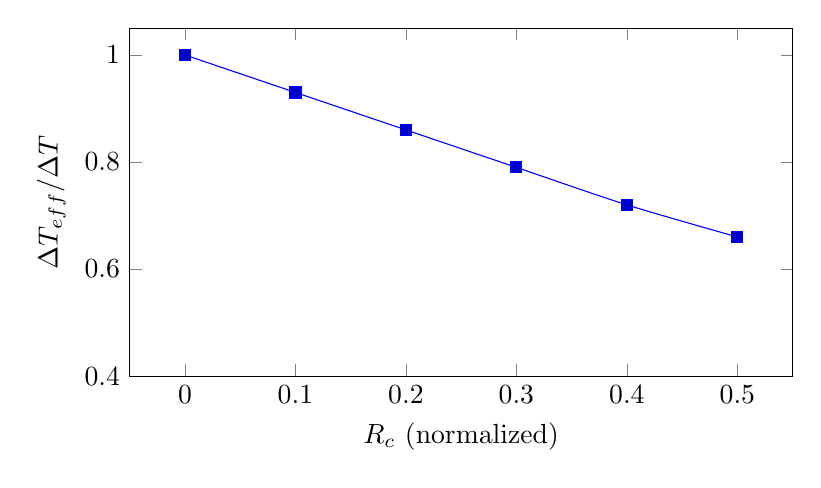
\begin{tikzpicture}
\begin{axis}[width=10cm,height=6cm,xlabel={$R_c$ (normalized)},ylabel={$\Delta T_{eff}/\Delta T$},ymin=0.4,ymax=1.05]
\addplot+[smooth,mark=square*] coordinates {(0,1.0)(0.1,0.93)(0.2,0.86)(0.3,0.79)(0.4,0.72)(0.5,0.66)};
\end{axis}
\end{tikzpicture}
\caption{Impact of contact resistance on effective temperature gradient.}
\label{fig:contact_resistance}
\end{figure}

\begin{table}[htbp]
\centering
\caption{Representative thermoelectric transport symbols and implications.}
\label{tab:te_symbols}
\begin{tabular}{lll}
\toprule
Parameter & Meaning & Design implication \\
\midrule
$S$ & Thermopower & Increase voltage response \\
$\sigma$ & Carrier transport & Reduce Joule losses \\
$\kappa_l$ & Phonon heat leakage & Suppress via scattering \\
$R_c$ & Contact resistance & Preserve usable $\Delta T$ \\
\bottomrule
\end{tabular}
\end{table}
